\subsection{Kỹ thuật Thiết kế Đặc trưng (Feature Engineering \& Justification)}
\label{sec:5_2}

Dữ liệu thô thu thập từ mạng lưới cảm biến giao thông thường chứa nhiều độ trễ, nhiễu và các điểm khuyết thiếu (missing values). Do đó, để mô hình học máy – đặc biệt là mạng nơ-ron chuỗi thời gian – có thể hội tụ và trích xuất quy luật hiệu quả, dữ liệu thô cần được biến đổi thành các vector đặc trưng mang ý nghĩa vật lý. Mục này trình bày các kỹ thuật nền tảng để cấu trúc hóa không gian trạng thái từ dòng dữ liệu thô.

\subsubsection{Cấu trúc Cửa sổ trượt (Sliding Window) và Đảm bảo tính liên tục (Continuity)}

Bài toán dự báo giao thông không xem xét từng điểm dữ liệu đơn lẻ mà đánh giá chuỗi diễn biến trong quá khứ để suy luận tương lai. Để định dạng dữ liệu cho mô hình chuỗi thời gian (như LSTM), hệ thống sử dụng kỹ thuật Cửa sổ trượt (Sliding Window).

\paragraph{a. Thông số và Biện luận kích thước cửa sổ (Window Size Justification)}
Hệ thống thiết lập kích thước cửa sổ $W = 12$ bước thời gian (time-steps). Với tần suất thu thập dữ liệu (Aggregation resolution) là $15$ phút/bước, kích thước cửa sổ này tương đương với $3$ giờ đồng hồ lịch sử.

\textbf{Cơ sở lựa chọn:} Việc chọn $3$ giờ không phải là ngẫu nhiên mà dựa trên đặc tính lan truyền của dòng xe. Kẹt xe đô thị không xảy ra tức thời mà phát triển theo dạng "sóng xung kích" (Shockwaves). Một khoảng thời gian 3 giờ là vừa đủ để mô hình quan sát trọn vẹn một chu kỳ chuyển dịch trạng thái: từ giai đoạn giao thông bắt đầu ùn ứ tích lũy, đạt đỉnh điểm vỡ trận (bottleneck), cho đến khi dòng xe bắt đầu giải phóng.
\begin{itemize}
    \item Nếu chọn cửa sổ quá ngắn (ví dụ 30 phút), mô hình sẽ thiếu "tầm nhìn" dài hạn để nhận biết xu hướng.
    \item Nếu chọn cửa sổ quá dài (ví dụ 6 giờ), dữ liệu sẽ chứa nhiều thông tin nhiễu từ các khung giờ không liên quan, làm giảm hiệu suất tính toán của bộ nhớ hệ thống.
\end{itemize}
Cửa sổ này sẽ trích xuất một chuỗi đầu vào $X = [x_{t-11}, x_{t-10}, \dots, x_t]$ để dự báo nhãn mục tiêu $Y = y_{t+1}$ (dự báo trước 15 phút).

\paragraph{b. Thuật toán kiểm soát tính liên tục (Continuity Check Algorithm)} \mbox{} \\
Một thách thức lớn của dữ liệu IoT (Internet of Things) ngoài thực tế là hiện tượng rớt mạng, mất tín hiệu cảm biến, dẫn đến các "lỗ hổng" thời gian trong cơ sở dữ liệu. Nếu hệ thống áp dụng cửa sổ trượt một cách mù quáng, cửa sổ có thể chứa những dòng dữ liệu đứt gãy (ví dụ: nhảy vọt từ 08:00 sáng thẳng đến 14:00 chiều do mất kết nối). Việc đưa một chuỗi đứt gãy không gian thời gian vào mô hình LSTM sẽ gây ra sự sai lệch nghiêm trọng về mặt nhận thức động lực học.

Để khắc phục, đồ án thiết kế thuật toán \textbf{Kiểm tra tính liên tục} (\texttt{find\_valid\_window\_starts}). Thuật toán này hoạt động như một màng lọc nghiêm ngặt:
\begin{enumerate}
    \item Quét qua trục thời gian và kiểm tra khoảng cách (delta) giữa mọi điểm dữ liệu liên tiếp trong cửa sổ $W+1$ (bao gồm cả điểm mục tiêu).
    \item Chỉ những cửa sổ thỏa mãn điều kiện khoảng cách thời gian giữa các bước chính xác tuyệt đối bằng 15 phút (không chứa giá trị NaN hoặc bước nhảy vọt) mới được gán cờ hợp lệ (Valid).
    \item Các cửa sổ vi phạm sẽ bị loại bỏ hoàn toàn nhằm bảo vệ tính toàn vẹn (Data Integrity) của tập huấn luyện. Kỹ thuật này đóng vai trò then chốt giúp Agent Học tăng cường không bị học sai các quy luật vật lý nhân quả.
\end{enumerate}

\begin{figure}[H]
    \centering
    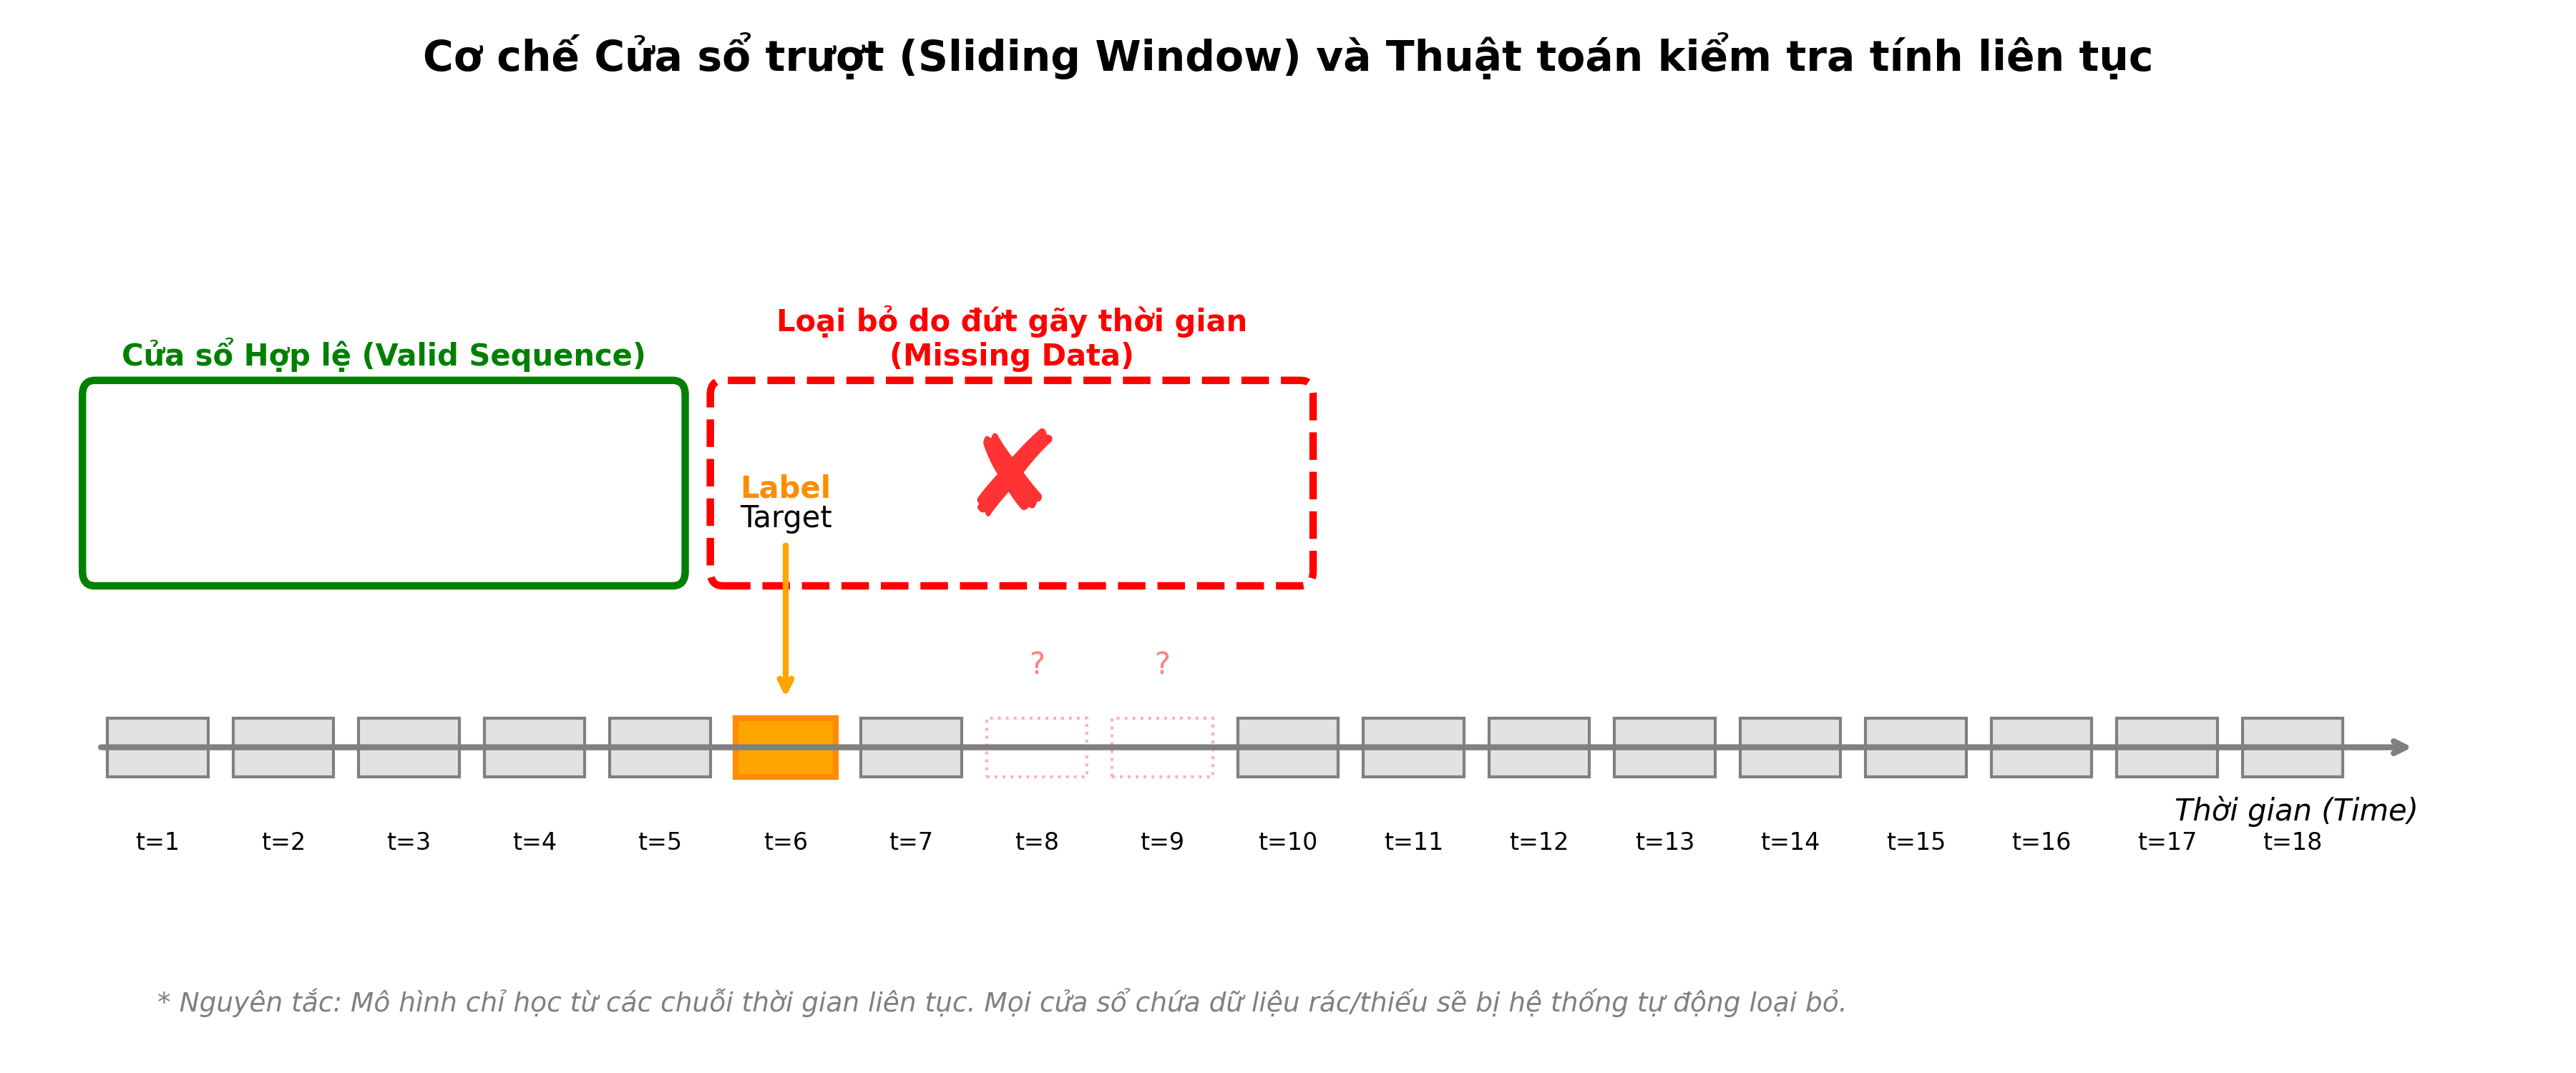
\includegraphics[width=0.8\textwidth]{Images/CH5/6.png}
    \vspace{12pt}
    \caption{Sơ đồ minh họa cơ chế Cửa sổ trượt và Thuật toán kiểm tra tính liên tục}
    \label{fig:5_6}
\end{figure}

\subsubsection{Nhúng bối cảnh không gian (Spatial \& Categorical Embedding)}

Trong mạng lưới giao thông thực tế, các đặc trưng mang tính định danh không gian như Mã đoạn đường (segment\_id) hay Mã khu vực (ward\_id) đóng vai trò là "bối cảnh" cực kỳ quan trọng. Cùng một mức vận tốc 20 km/h, nhưng tại một con hẻm nhỏ thì đó là trạng thái lưu thông bình thường, trong khi tại một đại lộ lớn thì đó là dấu hiệu của ùn tắc nghiêm trọng. Để mô hình hiểu được bối cảnh này, các biến phân loại (categorical variables) cần được chuyển đổi thành biểu diễn toán học.

\paragraph{a. Hạn chế của One-hot Encoding và "Lời nguyền số chiều"} \mbox{} \\
Phương pháp truyền thống thường được sử dụng cho dữ liệu phân loại là One-hot Encoding. Tuy nhiên, khi áp dụng vào bài toán mạng lưới giao thông diện rộng, phương pháp này bộc lộ hai lỗ hổng chí mạng:
\begin{enumerate}
    \item \textbf{Lời nguyền số chiều (Curse of Dimensionality):} Nếu mạng lưới có 500 đoạn đường, One-hot Encoding sẽ tạo ra một vector có 500 chiều cho mỗi điểm dữ liệu, trong đó chỉ có một giá trị $1$ và $499$ giá trị $0$. Điều này tạo ra một "ma trận thưa" (Sparse Matrix) khổng lồ, làm cạn kiệt bộ nhớ RAM, gây ra hiện tượng tiêu biến đạo hàm (Vanishing Gradient) và làm chậm tốc độ hội tụ của thuật toán DQN một cách nghiêm trọng.
    \item \textbf{Sự trực giao vô nghĩa về mặt không gian:} Về mặt toán học, One-hot Encoding giả định tất cả các đoạn đường đều hoàn toàn độc lập và trực giao với nhau. Khoảng cách (Euclidean hoặc Cosine) giữa đoạn đường A và đoạn đường B luôn bằng với khoảng cách từ A đến C. Điều này vi phạm hoàn toàn quy luật vật lý giao thông, nơi các đoạn đường lân cận hoặc cùng tính chất sẽ có sự tương quan chặt chẽ với nhau.
\end{enumerate}

\paragraph{b. Kỹ thuật Nhúng (Embedding Layer) và Chiều không gian} \mbox{} \\
Để giải quyết triệt để vấn đề trên, đồ án tích hợp \textbf{Tầng Nhúng (Embedding Layer)} vào mạng nơ-ron để xử lý các ID không gian. Kỹ thuật này ánh xạ một tập hợp rời rạc, phân tán thành một không gian vector đặc (Dense Vector Space) có số chiều thấp và mang tính liên tục.

Hệ thống thiết lập siêu tham số kích thước không gian nhúng là $Embedding Dimension = 8$. Kích thước 8 chiều được lựa chọn thông qua thực nghiệm (Empirical tuning) vì nó đóng vai trò là "Điểm vàng" (Sweet spot):
\begin{itemize}
    \item Đủ lớn để mô hình có dung lượng đại diện (representational capacity) nhằm mã hóa các đặc tính hình học phức tạp của đoạn đường.
    \item Đủ nhỏ để không làm bùng nổ số lượng tham số huấn luyện, tránh hiện tượng học vẹt (Overfitting) trên dữ liệu nhiễu.
\end{itemize}

\paragraph{c. Tác dụng: Mô hình hóa "Khoảng cách Giao thông"} \mbox{} \\
Sức mạnh lớn nhất của tầng Embedding nằm ở khả năng tự học (Self-learning). Ban đầu, các vector 8 chiều được khởi tạo ngẫu nhiên. Trải qua hàng ngàn vòng lặp huấn luyện lan truyền ngược (Backpropagation), trọng số của các vector này liên tục được tinh chỉnh để tối ưu hóa hàm mất mát (Loss function) dự báo kẹt xe.

Kết quả là, mô hình tự động xây dựng được một "Bản đồ nhận thức" về \textbf{Khoảng cách giao thông (Traffic Distance)} thay vì khoảng cách địa lý đơn thuần. Trong không gian 8 chiều này:
\begin{itemize}
    \item Các đoạn đường tuy cách xa nhau về mặt địa lý nhưng có cùng chức năng giao thông (ví dụ: cùng là nút giao thông thường xuyên xảy ra xung đột rẽ trái, hoặc cùng là đường nhánh nối ra xa lộ) sẽ có các vector nhúng "hội tụ" về gần nhau.
    \item Các đoạn đường lân cận nằm trên cùng một trục hành lang giao thông (Corridor) sẽ chia sẻ các cụm vector tương đồng, giúp Agent nội suy được trạng thái ùn tắc lan truyền từ đoạn đường này sang đoạn đường khác một cách tự nhiên.
\end{itemize}
Nhờ kỹ thuật này, hệ thống dự báo không chỉ nhìn thấy dữ liệu dưới dạng những con số rời rạc, mà thực sự "hiểu" được cấu trúc địa hình học và động lực học ẩn của toàn mạng lưới đường bộ.

\begin{figure}[H]
    \centering
    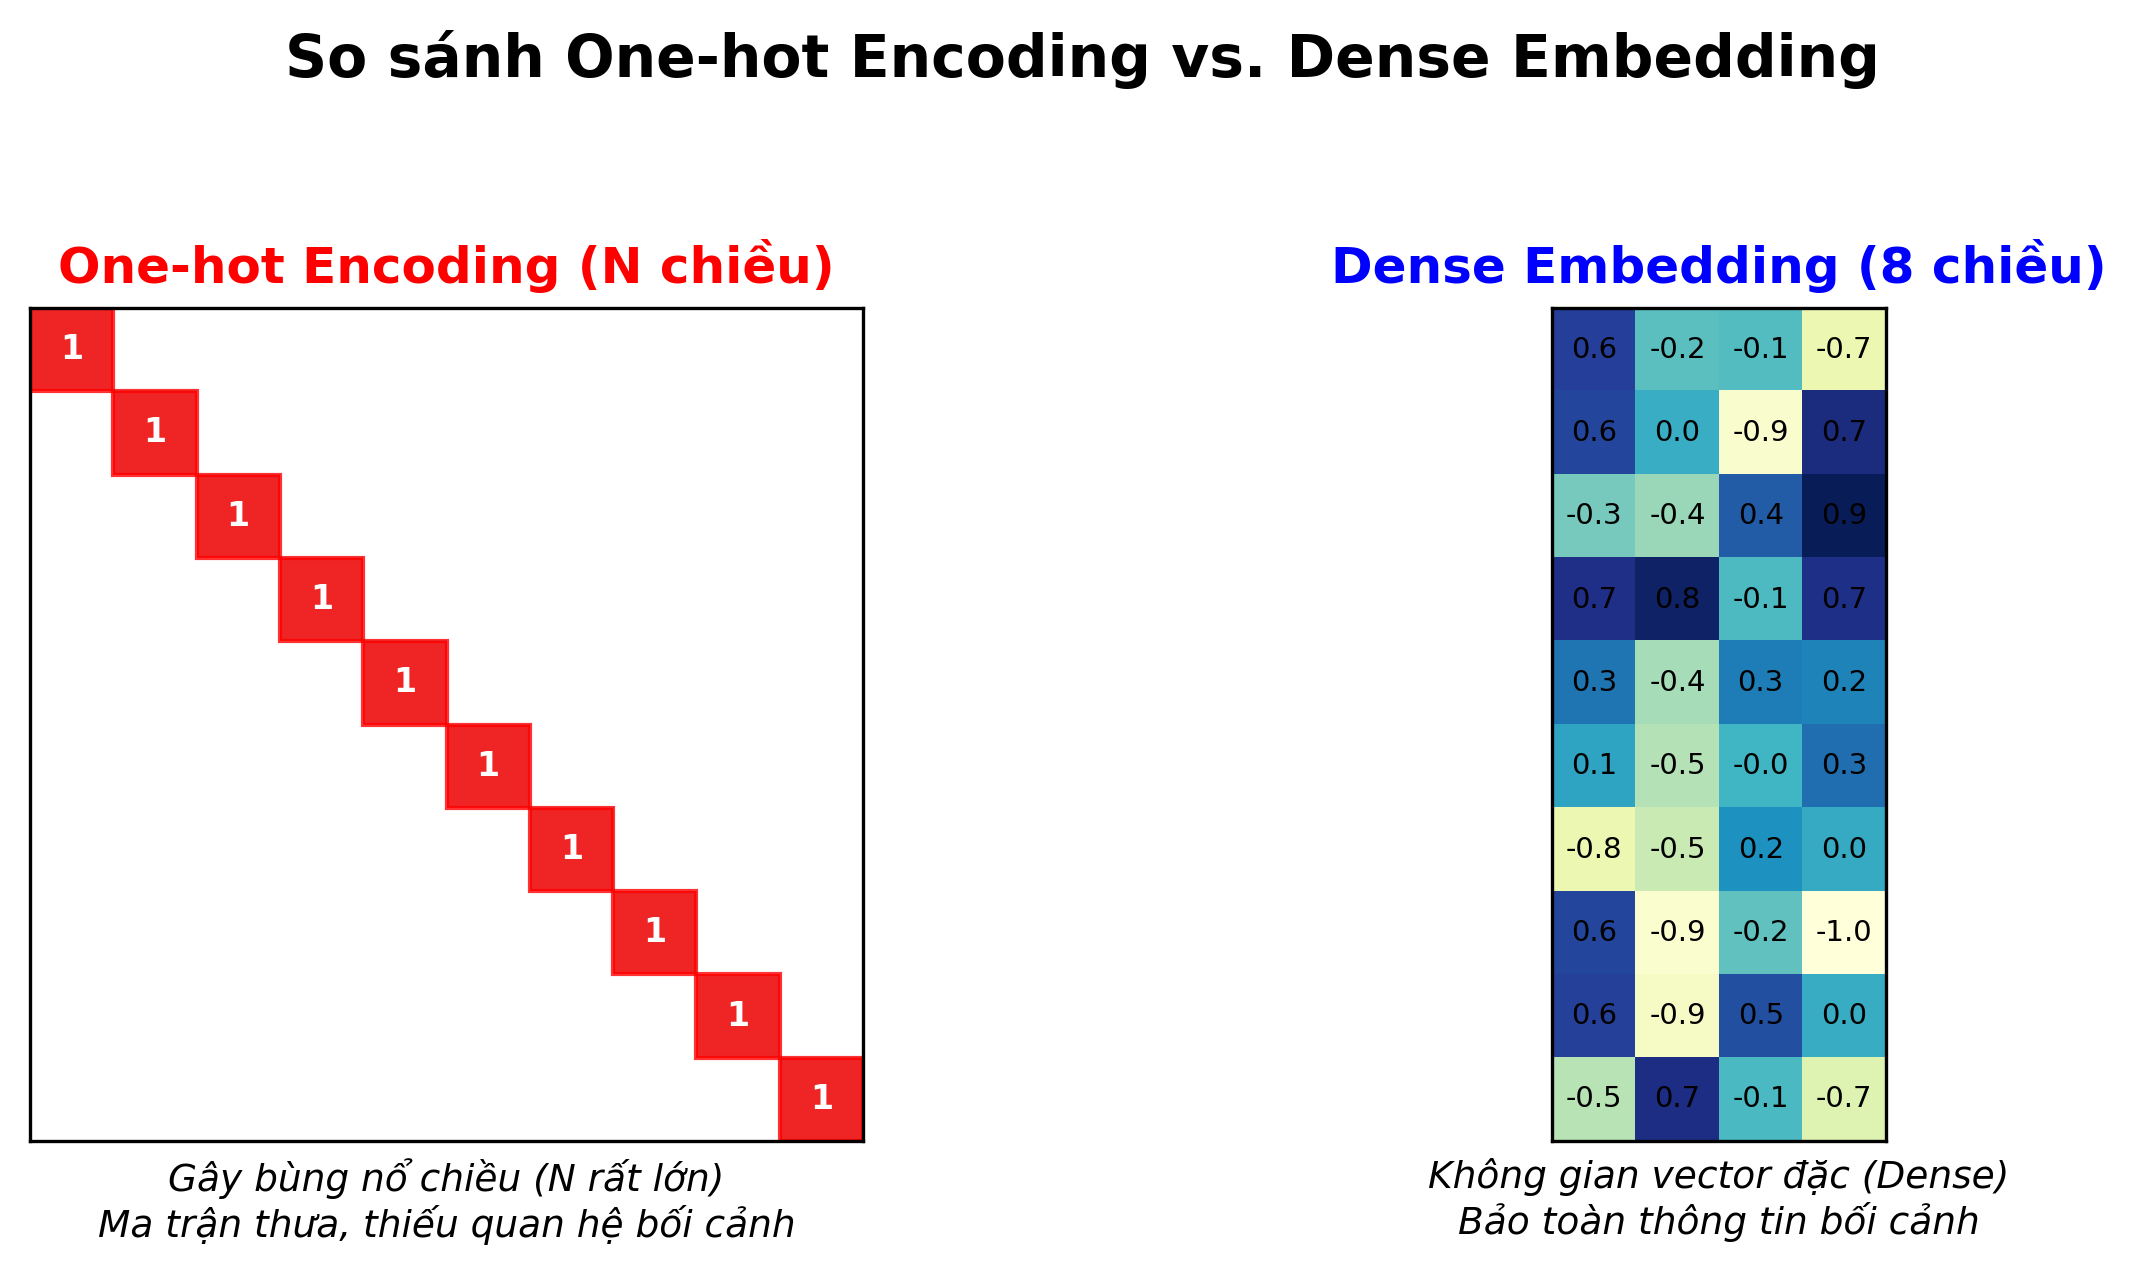
\includegraphics[width=0.8\textwidth]{Images/CH5/7.png}
    \vspace{12pt}
    \caption{So sánh One-hot Encoding vs Dense Embedding}
    \label{fig:5_7}
\end{figure}

\subsubsection{Mã hóa tính chu kỳ thời gian (Cyclical Temporal Encoding)}

Lưu lượng và tình trạng giao thông đô thị mang tính chu kỳ (Seasonality) cực kỳ rõ rệt, lặp đi lặp lại theo nhịp sinh học của con người (như chu kỳ ngày đêm, chu kỳ tuần làm việc). Do đó, "Thời gian trong ngày" (Time of day) là một trong những đặc trưng quan trọng nhất để dự báo kẹt xe. Tuy nhiên, cách biểu diễn dữ liệu thời gian thô vào mô hình học máy quyết định trực tiếp đến tốc độ và khả năng hội tụ của hệ thống.

\paragraph{a. Hạn chế của mã hóa tuyến tính (Linear / Ordinal Encoding)} \mbox{} \\
Cách tiếp cận thông thường là biểu diễn thời gian (Giờ) dưới dạng số nguyên tuyến tính từ $0$ đến $23$. Dưới góc độ tối ưu hóa của mạng nơ-ron, cách mã hóa này tạo ra một \textbf{khoảng cách giả tạo (Artificial Distance)} cực kỳ nguy hiểm:
\begin{itemize}
    \item Về mặt toán học, khoảng cách giữa $23$ (23:00 đêm) và $0$ (00:00 sáng hôm sau) là $\Delta = |23 - 0| = 23$.
    \item Về mặt vật lý giao thông, 23:59 và 00:01 là hai thời điểm liền kề nhau, trạng thái giao thông gần như không thay đổi.
\end{itemize}
Sự đứt gãy tuyến tính này (bước nhảy đột ngột từ 23 về 0) tạo ra một bề mặt dốc gồ ghề (Loss landscape discontinuities) trong không gian đặc trưng. Thuật toán Gradient Descent sẽ phải tốn rất nhiều chu kỳ (epochs) chỉ để học cách "bẻ cong" logic toán học nhằm bù đắp cho sự vô lý này, làm giảm hiệu suất của mô hình.

\paragraph{b. Kỹ thuật Mã hóa Chu kỳ bằng hàm Lượng giác (Sin/Cos Transformation)} \mbox{} \\
Để giải quyết triệt để sự đứt gãy, đồ án áp dụng kỹ thuật \textbf{Mã hóa Chu kỳ (Cyclical Temporal Encoding)}. Kỹ thuật này chiếu trục thời gian tuyến tính 1 chiều lên một đường tròn đơn vị 2 chiều, thông qua hai hàm lượng giác hình sin và cô-sin.

Với $t$ là thời điểm hiện tại (tính bằng phút hoặc giờ) và $T$ là tổng chu kỳ (ví dụ $T = 24$ đối với giờ, $T = 60$ đối với phút), đặc trưng thời gian được tách thành hai vector liên tục:
\begin{equation}
    \text{Time\_Sin} = \sin\left(\frac{2\pi \cdot t}{T}\right)
\end{equation}
\begin{equation}
    \text{Time\_Cos} = \cos\left(\frac{2\pi \cdot t}{T}\right)
\end{equation}

\textbf{Lý do phải sử dụng đồng thời cả Sin và Cos:} Nếu chỉ dùng hàm Sin, các thời điểm đối xứng qua trục tung (ví dụ 06:00 sáng và 18:00 chiều) sẽ cho ra cùng một giá trị, gây ra sự nhầm lẫn (Collision) cho Agent. Việc kết hợp cả hai hàm tạo ra một tọa độ $(x, y)$ duy nhất trên đường tròn cho mỗi phút trong ngày.

\paragraph{c. Lợi ích tối ưu hóa cho mô hình chuỗi thời gian}
Kỹ thuật này mang lại những ưu điểm vượt trội cho các cấu trúc mạng như LSTM hay Double DQN:
\begin{enumerate}
    \item \textbf{Bảo toàn khoảng cách vật lý:} Trong không gian không gian 2D mới, khoảng cách Euclidean giữa 23:59 và 00:01 tiệm cận về $0$, phản ánh chính xác sự liên tục của dòng chảy thời gian thực tế.
    \item \textbf{Làm mịn không gian đặc trưng (Feature space smoothing):} Việc loại bỏ các điểm gãy (discontinuities) giúp bề mặt hàm mất mát (Loss Function) trở nên trơn tru hơn. Mạng nơ-ron nhận được độ dốc (gradients) ổn định, từ đó tăng tốc độ hội tụ và giảm thiểu khả năng rơi vào cực tiểu cục bộ (Local Minima) trong quá trình huấn luyện RL.
\end{enumerate}

\subsubsection{Chuẩn hóa và Tiền xử lý (Scaling \& Imputation)}

Trong kiến trúc của các hệ thống Học máy hiện đại, quá trình tiền xử lý không chỉ đơn thuần là bước làm sạch dữ liệu, mà là một trụ cột của quy trình MLOps nhằm đảm bảo tính ổn định toán học khi huấn luyện và tính nhất quán khi triển khai thực tế. Đồ án áp dụng một pipeline (đường ống) tiền xử lý nghiêm ngặt bao gồm các kỹ thuật sau:

\paragraph{a. Xử lý khuyết thiếu cục bộ (Local Imputation)} \mbox{} \\
Trong thực tiễn thu thập dữ liệu từ hệ thống cảm biến IoT giao thông, hiện tượng mất gói tin tạm thời (drop-out) diễn ra thường xuyên. Khác với các đứt gãy kéo dài (đã được xử lý bằng cách loại bỏ toàn bộ cửa sổ tại Mục 5.2.1), các khuyết thiếu cục bộ (chỉ mất tín hiệu trong 1-2 chu kỳ tương đương 15-30 phút) được giữ lại để tránh lãng phí dữ liệu.

Hệ thống áp dụng kỹ thuật \textbf{Điền khuyết tiến (Forward Fill - ffill)} để xử lý các lỗ hổng này. Cơ sở khoa học của phương pháp này dựa trên định luật quán tính vật lý của dòng xe: trong một khoảng thời gian cực ngắn, trạng thái động lực học của giao thông (vận tốc, mật độ) có xu hướng duy trì tính kế thừa từ thời điểm ngay trước đó. Việc lấy giá trị của $t_{i-1}$ đắp vào $t_i$ mang lại độ tin cậy cao hơn so với việc nội suy trung bình (mean imputation), đồng thời không phá vỡ tính nhân quả (causality) của chuỗi thời gian.

\paragraph{b. Cơ sở toán học của Chuẩn hóa đặc trưng (Feature Scaling)} \mbox{} \\
Dữ liệu giao thông đa phương thức chứa các đặc trưng có sự chênh lệch khổng lồ về mặt độ lớn (Magnitude):
\begin{itemize}
    \item Đặc trưng tuần hoàn (Time Sin/Cos): Bị giới hạn nghiêm ngặt trong đoạn $[-1, 1]$.
    \item Vận tốc (Speed): Dao động trong khoảng $[0, 80]$ km/h.
    \item Độ trễ thời gian (Delay): Có thể bùng nổ lên tới hàng ngàn giây ($> 3000$s).
\end{itemize}

Nếu đưa trực tiếp không gian đặc trưng thô này vào các mạng nơ-ron như LSTM, hệ thống sẽ rơi vào tình trạng \textbf{"Mù Nơ-ron" (Neuron Blindness)}. Khi đó, trọng số (weights) của các biến có độ lớn cao như Delay sẽ thống trị hoàn toàn luồng Gradient truyền ngược, trong khi các tín hiệu quan trọng nhưng có độ lớn nhỏ (như Time Sin/Cos) bị triệt tiêu hoàn toàn. Về mặt hình học tối ưu, sự chênh lệch này biến bề mặt hàm mất mát (Loss Landscape) thành một "khe núi" hẹp và sâu. Thuật toán Gradient Descent sẽ phải dao động (oscillation) liên tục theo đường zigzag tốn kém, dẫn đến hội tụ cực kỳ chậm hoặc mắc kẹt tại cực tiểu cục bộ.

Để giải quyết, đồ án áp dụng bộ biến đổi \textbf{StandardScaler}, chuẩn hóa các biến liên tục về phân phối chuẩn (với kỳ vọng $\mu = 0$ và độ lệch chuẩn $\sigma = 1$):
\begin{equation}
    x_{scaled} = \frac{x - \mu}{\sigma}
\end{equation}
Phép biến đổi này nắn chỉnh bề mặt hàm mất mát thành dạng lòng chảo đẳng hướng (Isotropic Bowl), cho phép vector Gradient hướng thẳng trực tiếp đến điểm cực tiểu toàn cục (Global Minimum), tối ưu hóa tốc độ học của Agent DQN.

\paragraph{c. Nguyên tắc cách ly chống Rò rỉ dữ liệu (Preventing Data Leakage)} \mbox{} \\
Một trong những sai lầm nghiêm trọng làm suy giảm tính minh bạch của các nghiên cứu AI là hiện tượng rò rỉ dữ liệu (Data Leakage) ở bước chuẩn hóa. Nếu tính toán $\mu$ và $\sigma$ trên toàn bộ tập dữ liệu trước khi phân chia, mô hình sẽ ngầm "nhìn trộm" thông tin phân phối của tương lai, dẫn đến kết quả đánh giá (F1-score, Accuracy) cao một cách ảo tưởng, nhưng lại thất bại thảm hại khi triển khai thực tế.

Để tuân thủ tiêu chuẩn khoa học, đồ án thiết lập quy trình cách ly tuyệt đối:
\begin{enumerate}
    \item Hàm \texttt{fit()} chỉ được thực thi duy nhất trên tập Huấn luyện (Training set) để trích xuất các tham số thống kê của "quá khứ".
    \item Các tham số $(\mu, \sigma)$ này lập tức được "đóng băng".
    \item Hàm \texttt{transform()} sử dụng các tham số đã đóng băng để biến đổi tập Kiểm định (Validation set) và tập Kiểm thử (Test set), đảm bảo mô hình đối mặt với dữ liệu kiểm thử hoàn toàn như một thực thể chưa từng quan sát.
\end{enumerate}

\paragraph{d. Đóng gói "Bản hợp đồng Dữ liệu" (Preprocessing Artifacts)} \mbox{} \\
Trong kiến trúc phần mềm thực tế, mô hình AI không hoạt động cô lập mà phải giao tiếp với các hệ thống ứng dụng phía người dùng. Để giải quyết bài toán chênh lệch môi trường (Environment Drift), toàn bộ bộ biến đổi (bao gồm StandardScaler và các LabelEncoder của nhánh Categorical) được hệ thống đóng gói thành một tệp nhị phân duy nhất mang tên \texttt{preprocessing\_artifacts.pkl}.

Tệp này hoạt động như một \textbf{"Bản hợp đồng Dữ liệu" (Data Contract)}. Khi hệ thống được triển khai lên Server (Deploy), mọi yêu cầu dự báo (Inference Request) gọi từ Ứng dụng di động truyền về đều bắt buộc phải đi qua tệp Artifacts này để chuẩn hóa. Cơ chế này đảm bảo luồng dữ liệu thời gian thực (Real-time data) từ API luôn được chiếu (project) vào đúng hệ quy chiếu không gian mà mô hình đã được huấn luyện, duy trì tính nhất quán tuyệt đối (Consistency) từ phòng thí nghiệm ra đến môi trường Production.

\begin{figure}[H]
    \centering
    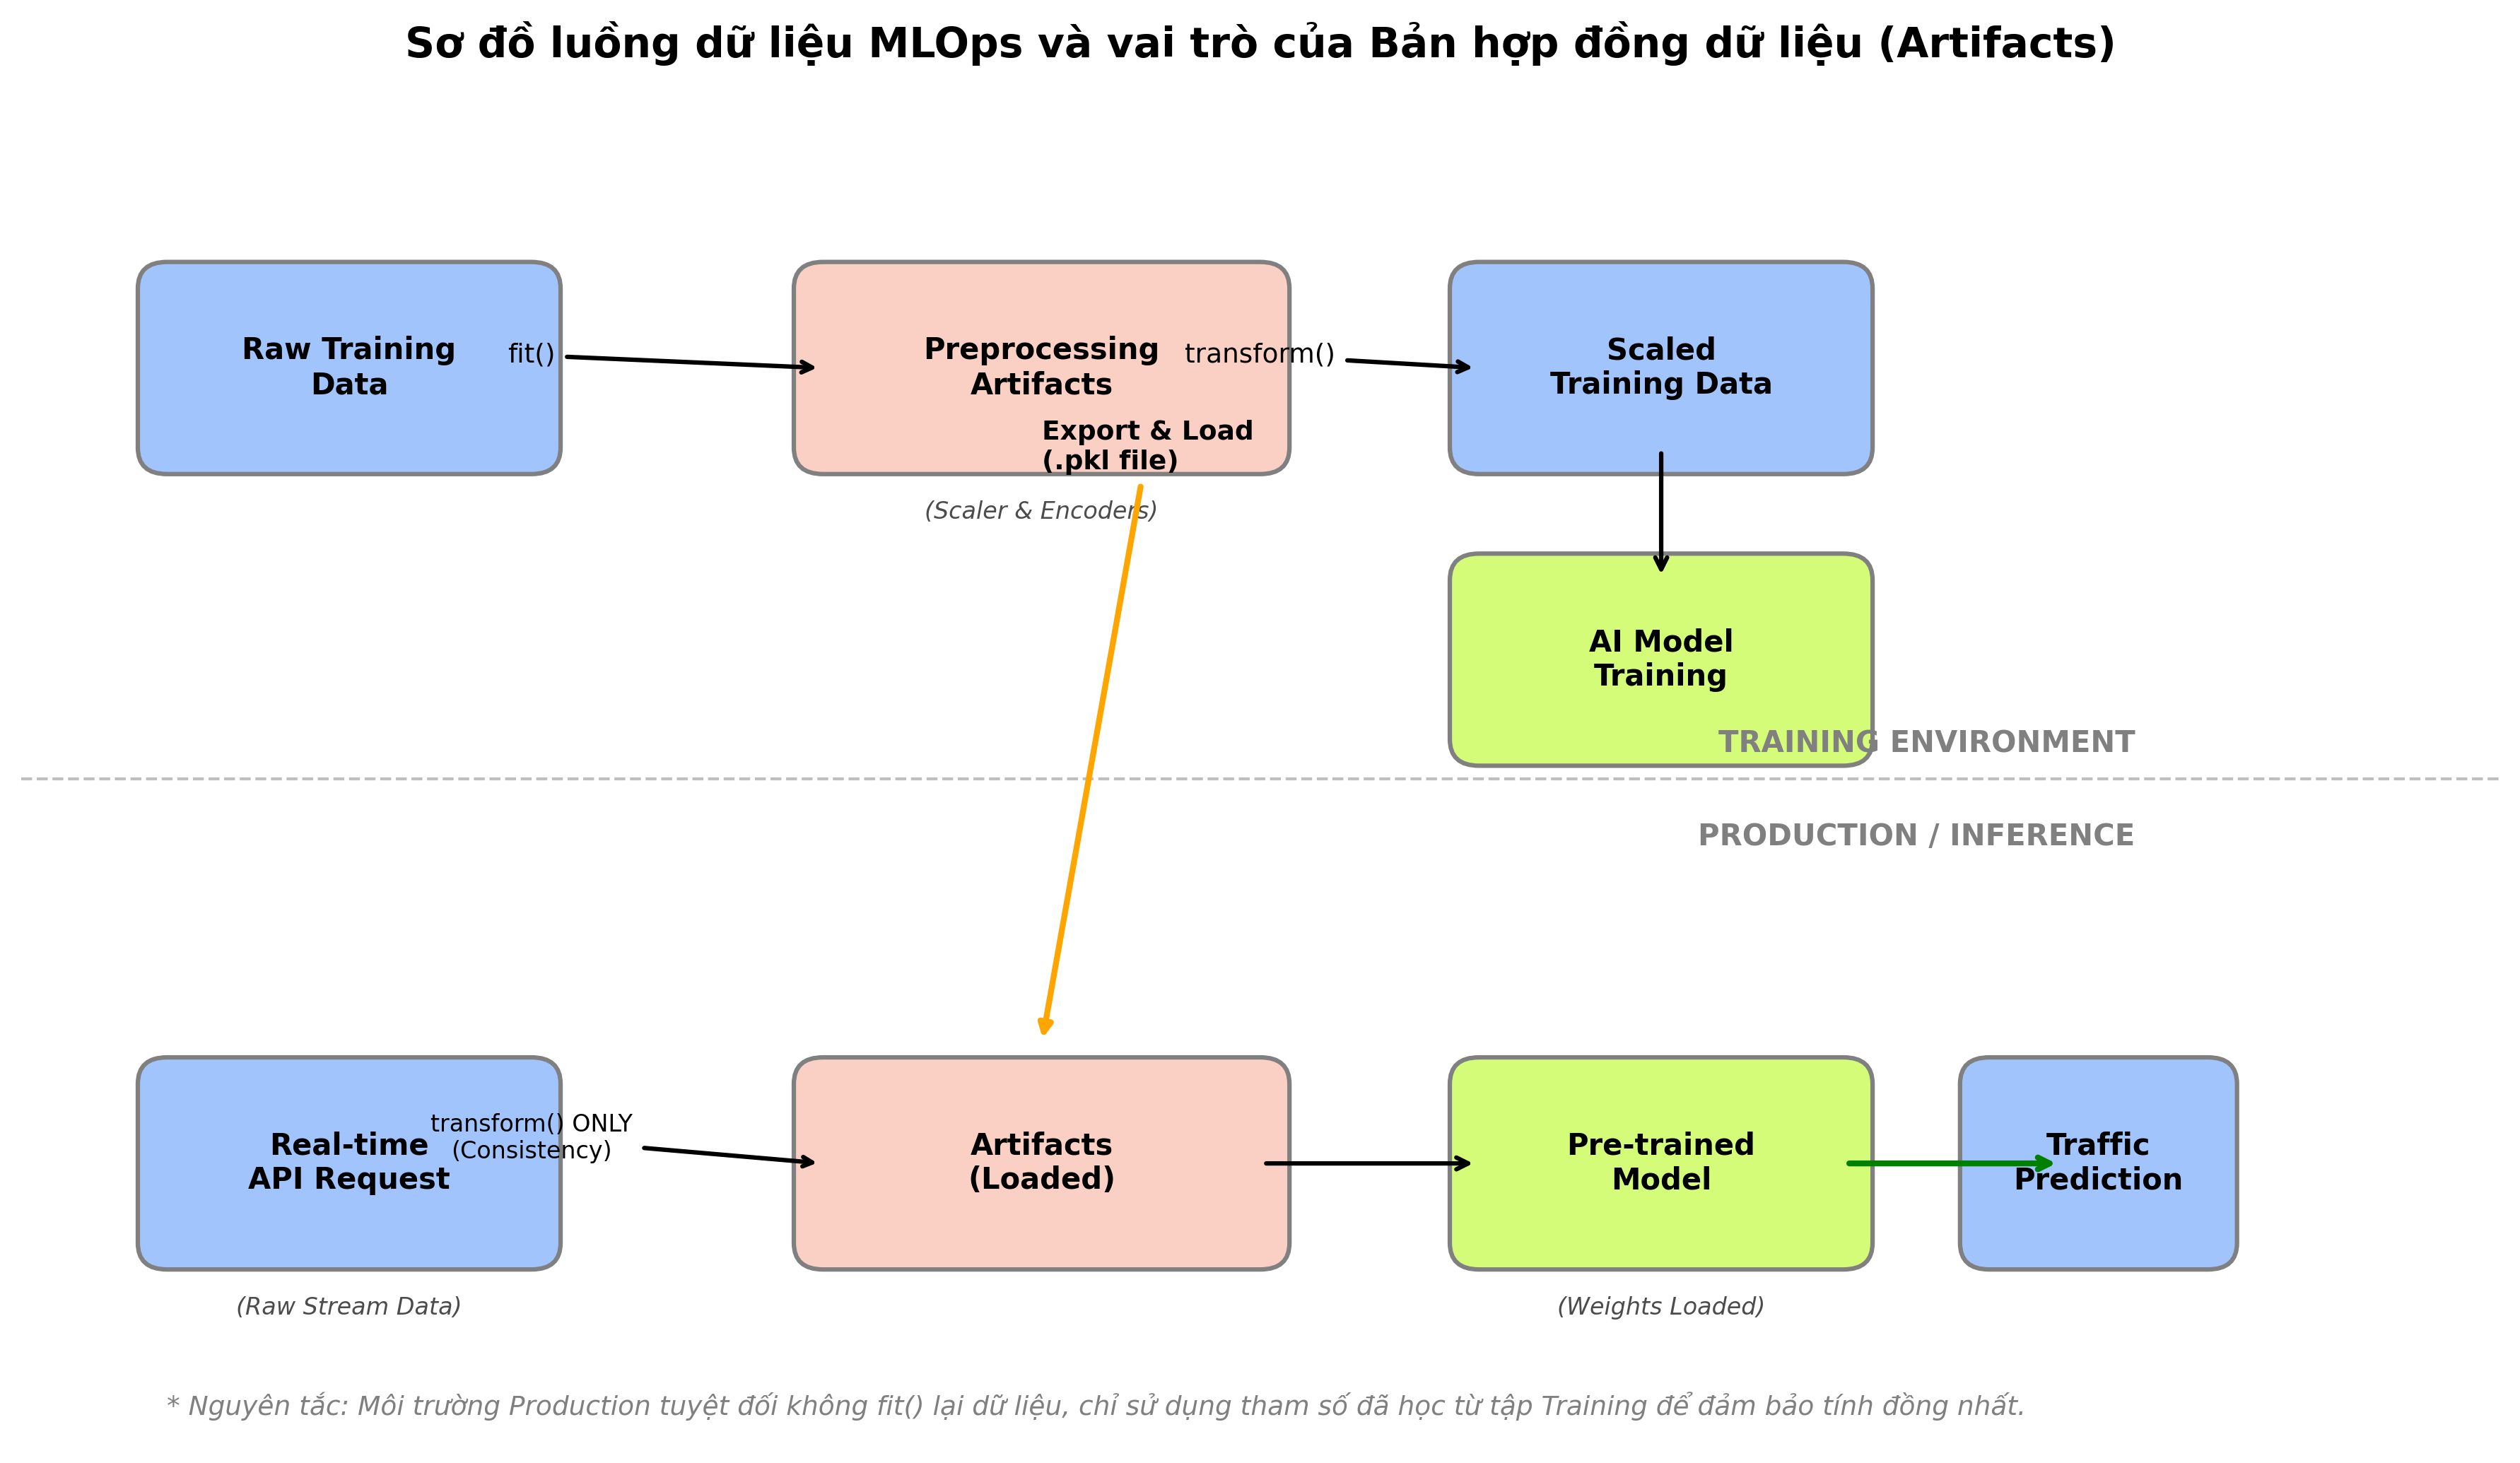
\includegraphics[width=0.8\textwidth]{Images/CH5/8.png}
    \vspace{12pt}
    \caption{Sơ đồ luồng dữ liệu MLOps}
    \label{fig:5_8}
\end{figure}

\subsubsection{Quy trình Đánh giá và Tuyển chọn Đặc trưng (Feature Quality Assessment)}

Trong thiết kế không gian trạng thái (State Space) cho mô hình Deep Learning và mạng Đặc vụ (RL Agent), việc "nhồi nhét" quá nhiều đặc trưng đầu vào không những không làm tăng hiệu suất mà còn dẫn đến hiện tượng "Lời nguyền số chiều" (Curse of Dimensionality). Càng nhiều chiều dữ liệu, không gian tìm kiếm càng phình to, tỷ lệ nhiễu (noise) tăng cao và bộ nhớ Replay Buffer sẽ nhanh chóng bị vắt kiệt.

Do đó, trước khi chốt danh sách đặc trưng cuối cùng đưa vào huấn luyện, đồ án thiết lập một quy trình tuyển chọn hai bước vô cùng nghiêm ngặt:

\paragraph{a. Bước 1 - Phân tích và Khử Đa cộng tuyến (Multicollinearity Removal)} \mbox{} \\
Đa cộng tuyến là hiện tượng hai hoặc nhiều đặc trưng đầu vào có mối tương quan tuyến tính quá mạnh với nhau. Ví dụ: Nếu hệ thống đã có đặc trưng \texttt{speed\_ratio} (tỷ lệ vận tốc hiện tại so với vận tốc tự do) thì việc giữ lại biến \texttt{avg\_speed} (vận tốc trung bình thô) là một sự dư thừa thông tin (Redundant features). Sự tồn tại của các biến dư thừa này sẽ khiến ma trận hiệp phương sai bị suy biến, làm cho trọng số của mạng Nơ-ron trở nên bất ổn định (instability) – một thay đổi nhỏ của dữ liệu đầu vào cũng làm Gradient nhảy vọt.

Để giải quyết, đồ án xây dựng \textbf{Ma trận tương quan Pearson/Spearman} phân tích chéo toàn bộ các biến. Hệ thống áp dụng một ngưỡng cắt cứng (Hard Threshold) là $0.7$. Bất kỳ cặp đặc trưng nào có hệ số tương quan tuyệt đối $|r| > 0.7$, hệ thống sẽ tự động đối chiếu với biến Mục tiêu (Target Label) và chỉ giữ lại biến nào có sức mạnh dự báo độc lập cao hơn, biến còn lại bị loại bỏ hoàn toàn khỏi pipeline.

Dựa trên kết quả thực nghiệm từ Ma trận tương quan, hệ thống đã phát hiện các cặp biến vi phạm nghiêm trọng giả định độc lập:
\begin{itemize}
    \item \textbf{Cặp \texttt{avg\_speed} và \texttt{speed\_ratio}:} Đạt hệ số tương quan dương cực đại $r = 0.97$. Điều này hoàn toàn hợp lý về mặt toán học vì tỷ lệ vận tốc được tính trực tiếp từ vận tốc trung bình. Việc giữ cả hai sẽ gây ra lỗi đa cộng tuyến hoàn hảo (Perfect Multicollinearity).
    \item \textbf{Cặp \texttt{traffic\_index} và \texttt{avg\_speed}:} Có độ tương quan âm rất mạnh $r = -0.89$. Khi vận tốc giảm sâu, chỉ số kẹt xe sẽ tăng vọt.
\end{itemize}

\textbf{Quyết định thiết kế:} Thay vì giữ toàn bộ, hệ thống áp dụng ngưỡng cắt tương quan $|r| > 0.85$. Đối với cặp (\texttt{avg\_speed}, \texttt{speed\_ratio}), đồ án quyết định chỉ giữ lại một đại diện có sức mạnh phân nhánh tốt hơn (được kiểm chứng ở Bước 2) để tối ưu hóa số chiều cho không gian vector đầu vào, giảm tải cho bộ nhớ Replay Buffer của Agent DQN.

\begin{figure}[H]
    \centering
    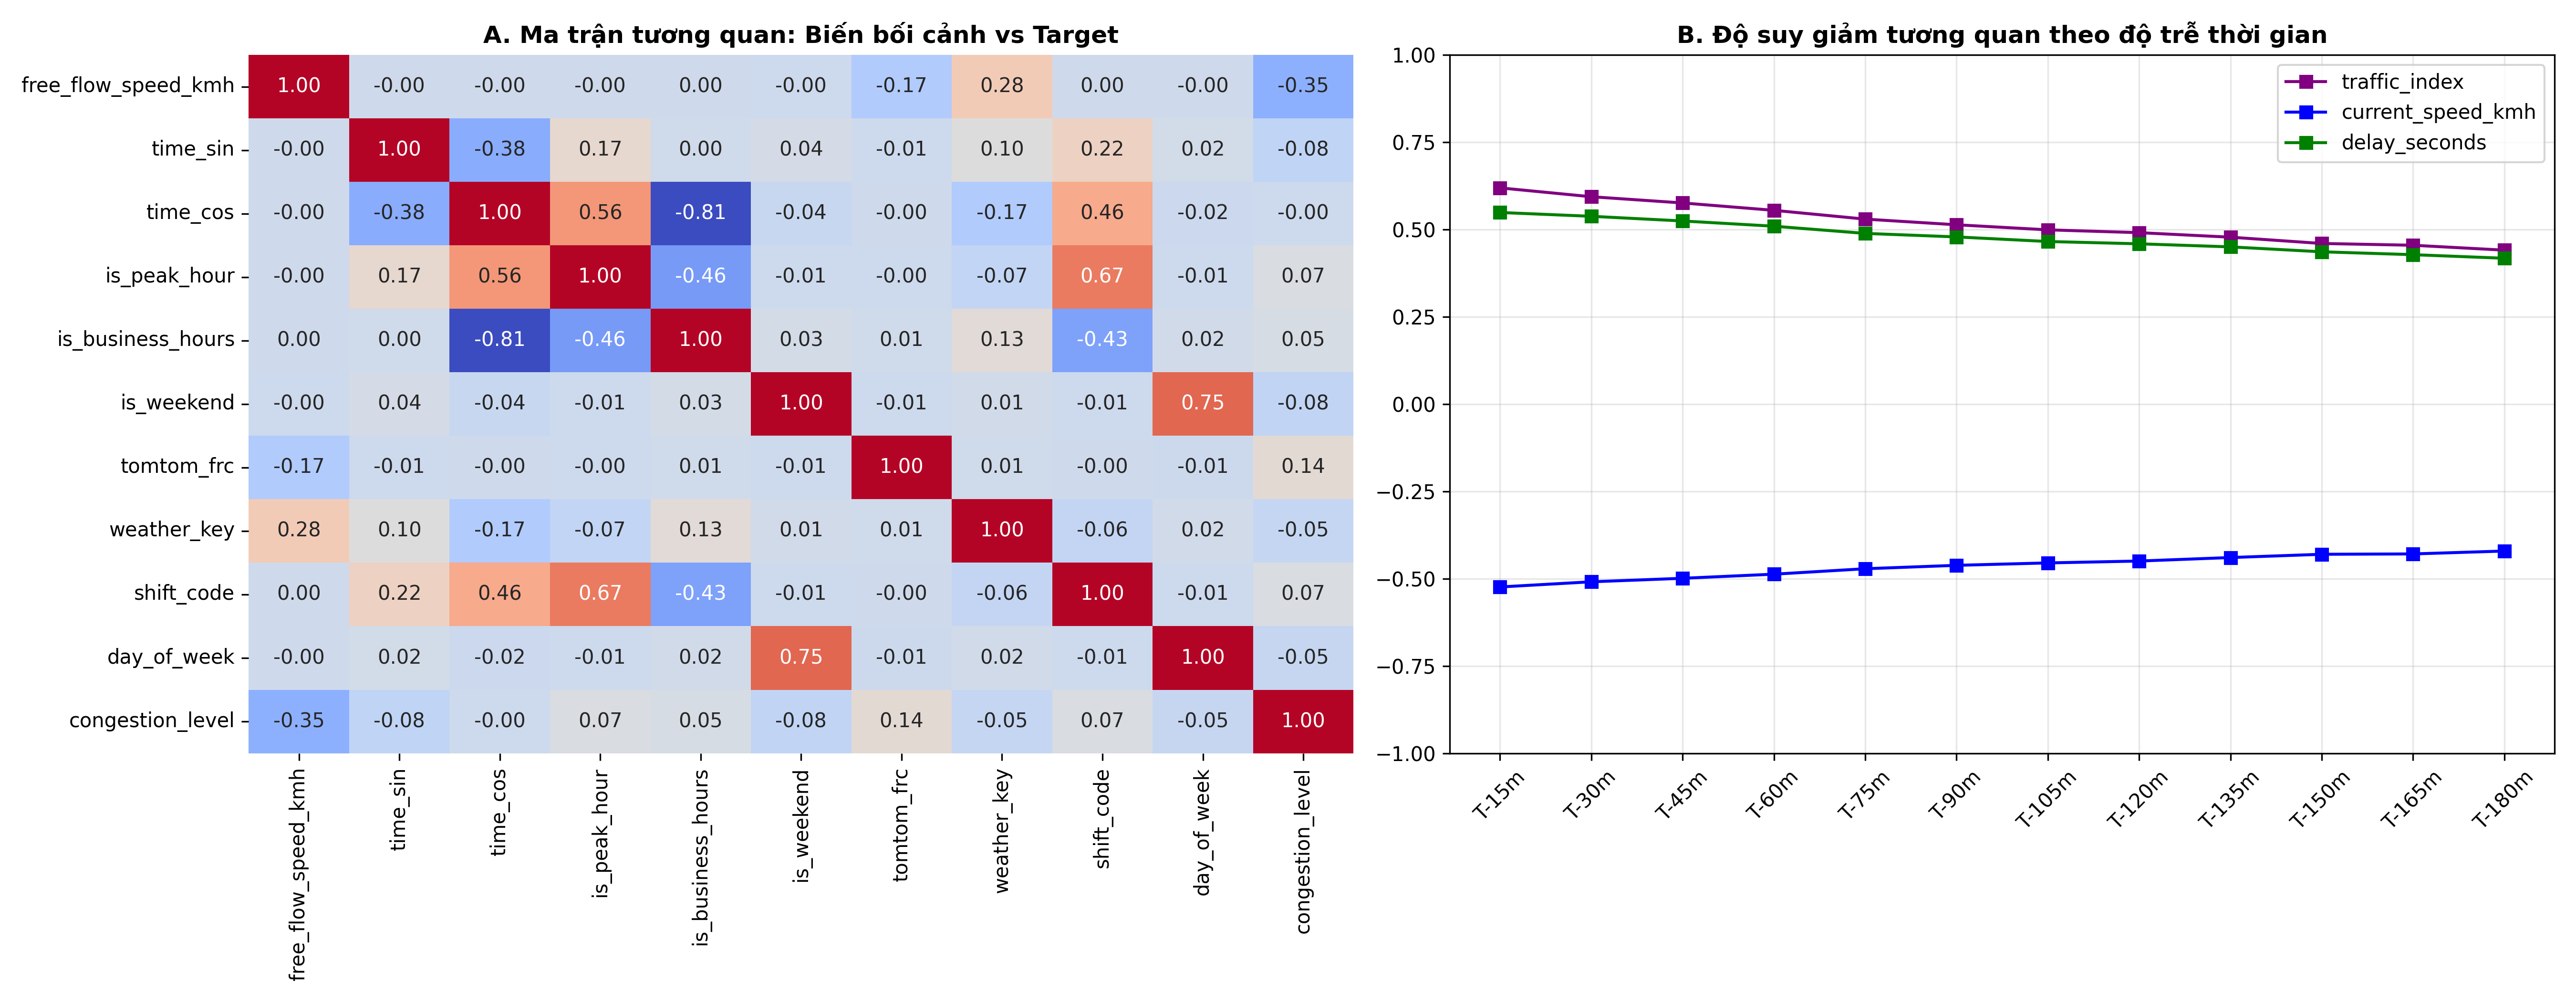
\includegraphics[width=0.8\textwidth]{Images/CH5/9.png}
    \vspace{12pt}
    \caption{Ma trận Tương quan (Heatmap) thể hiện hiện tượng đa cộng tuyến giữa các đặc trưng giao thông}
    \label{fig:5_9}
\end{figure}

\paragraph{b. Bước 2 - Xếp hạng Tầm quan trọng Đặc trưng (Feature Importance Ranking)} \mbox{} \\
Sau khi loại bỏ các biến dư thừa, những biến còn lại tiếp tục phải trải qua bài kiểm tra "Sức mạnh dự báo". Vì bản chất của giao thông là sự tương tác phi tuyến (ví dụ: mưa to + giờ cao điểm = kẹt xe vỡ trận), các phương pháp kiểm định thống kê tuyến tính thông thường (như Anova) sẽ không thể đánh giá đúng vai trò của từng biến.

Đồ án sử dụng thuật toán \textbf{Random Forest (Rừng ngẫu nhiên)} kết hợp với kỹ thuật kiểm chứng chéo \textbf{Stratified K-Fold} để xếp hạng đặc trưng.
\begin{itemize}
    \item \textbf{Lý do dùng Random Forest:} Thuật toán này có khả năng tự động tính toán chỉ số Gini Importance (hoặc Mean Decrease Impurity) bằng cách đo lường mức độ giảm nhiễu thông tin (Entropy) mỗi khi một đặc trưng được chọn để phân nhánh cây quyết định.
    \item \textbf{Lý do dùng Stratified K-Fold:} Vì phân phối nhãn kẹt xe đang mất cân bằng cực hạn (Thảm họa lớp 5 chỉ chiếm $< 1\%$), kỹ thuật Stratified (Phân tầng) đảm bảo rằng trong bất kỳ tập kiểm chứng nào, tỷ lệ các ca thảm họa vẫn được duy trì. Điều này ép thuật toán Random Forest phải đánh giá tầm quan trọng của đặc trưng dựa trên khả năng phát hiện thảm họa, chứ không chỉ dựa trên nhóm đa số.
\end{itemize}

Kết quả trích xuất từ Biểu đồ Xếp hạng Đặc trưng (Hình \ref{fig:5_10}) cho thấy sự phân hóa cực kỳ rõ nét thành 3 nhóm tín hiệu:
\begin{enumerate}
    \item \textbf{Nhóm Tín hiệu Cốt lõi (Core Signals):} Đóng vai trò thống trị tuyệt đối trong việc phát hiện kẹt xe. Dẫn đầu là \texttt{traffic\_index} với mức đóng góp áp đảo $\sim 40\%$, tiếp theo là \texttt{delay\_seconds} ($\sim 25\%$) và \texttt{avg\_speed} ($\sim 12\%$). Nhóm này phản ánh trực tiếp động lực học của "sóng xung kích" giao thông. Đây cũng là lý do ở Bước 1, biến \texttt{avg\_speed} chứng minh được giá trị giữ lại cao hơn \texttt{speed\_ratio} (chỉ đạt $\sim 5\%$).
    \item \textbf{Nhóm Bối cảnh Động (Contextual Signals):} Bao gồm \texttt{is\_rush\_hour} (Giờ cao điểm), \texttt{weather\_condition\_id} (Thời tiết), và tính chu kỳ \texttt{time\_sin}, \texttt{time\_cos}. Dù chỉ đóng góp mức nhỏ ($2\% - 4\%$ mỗi biến), nhưng đây là các biến "công tắc" cực kỳ quan trọng. Mạng Nơ-ron kết hợp chúng với nhóm cốt lõi để nhận diện các vụ kẹt xe thảm họa do mưa bão hoặc tan tầm.
    \item \textbf{Nhóm Vùng Nhiễu/Tĩnh (Static Noise):} Các thuộc tính vật lý tĩnh như \texttt{lanes} (Số làn xe) và \texttt{road\_length} (Chiều dài đoạn đường) nằm ở vị trí chót bảng với mức đóng góp $< 1\%$. Vì chúng không biến thiên theo thời gian, thuật toán cây quyết định không thể dùng chúng để rẽ nhánh cảnh báo. Tuy nhiên, thay vì loại bỏ hoàn toàn, hệ thống đã khôn khéo đẩy các ID định danh không gian này vào Tầng Nhúng (Embedding Layer) (như đã trình bày ở Mục 5.2.2) để học bối cảnh chìm, thay vì dùng làm chuỗi tín hiệu thời gian trực tiếp.
\end{enumerate}

Quy trình chắt lọc khắt khe này giúp Agent DQN của đồ án "nhẹ gánh" tính toán, tập trung toàn bộ tài nguyên mạng Nơ-ron vào những tín hiệu mang tính quyết định sinh tử của bài toán.

\begin{figure}[H]
    \centering
    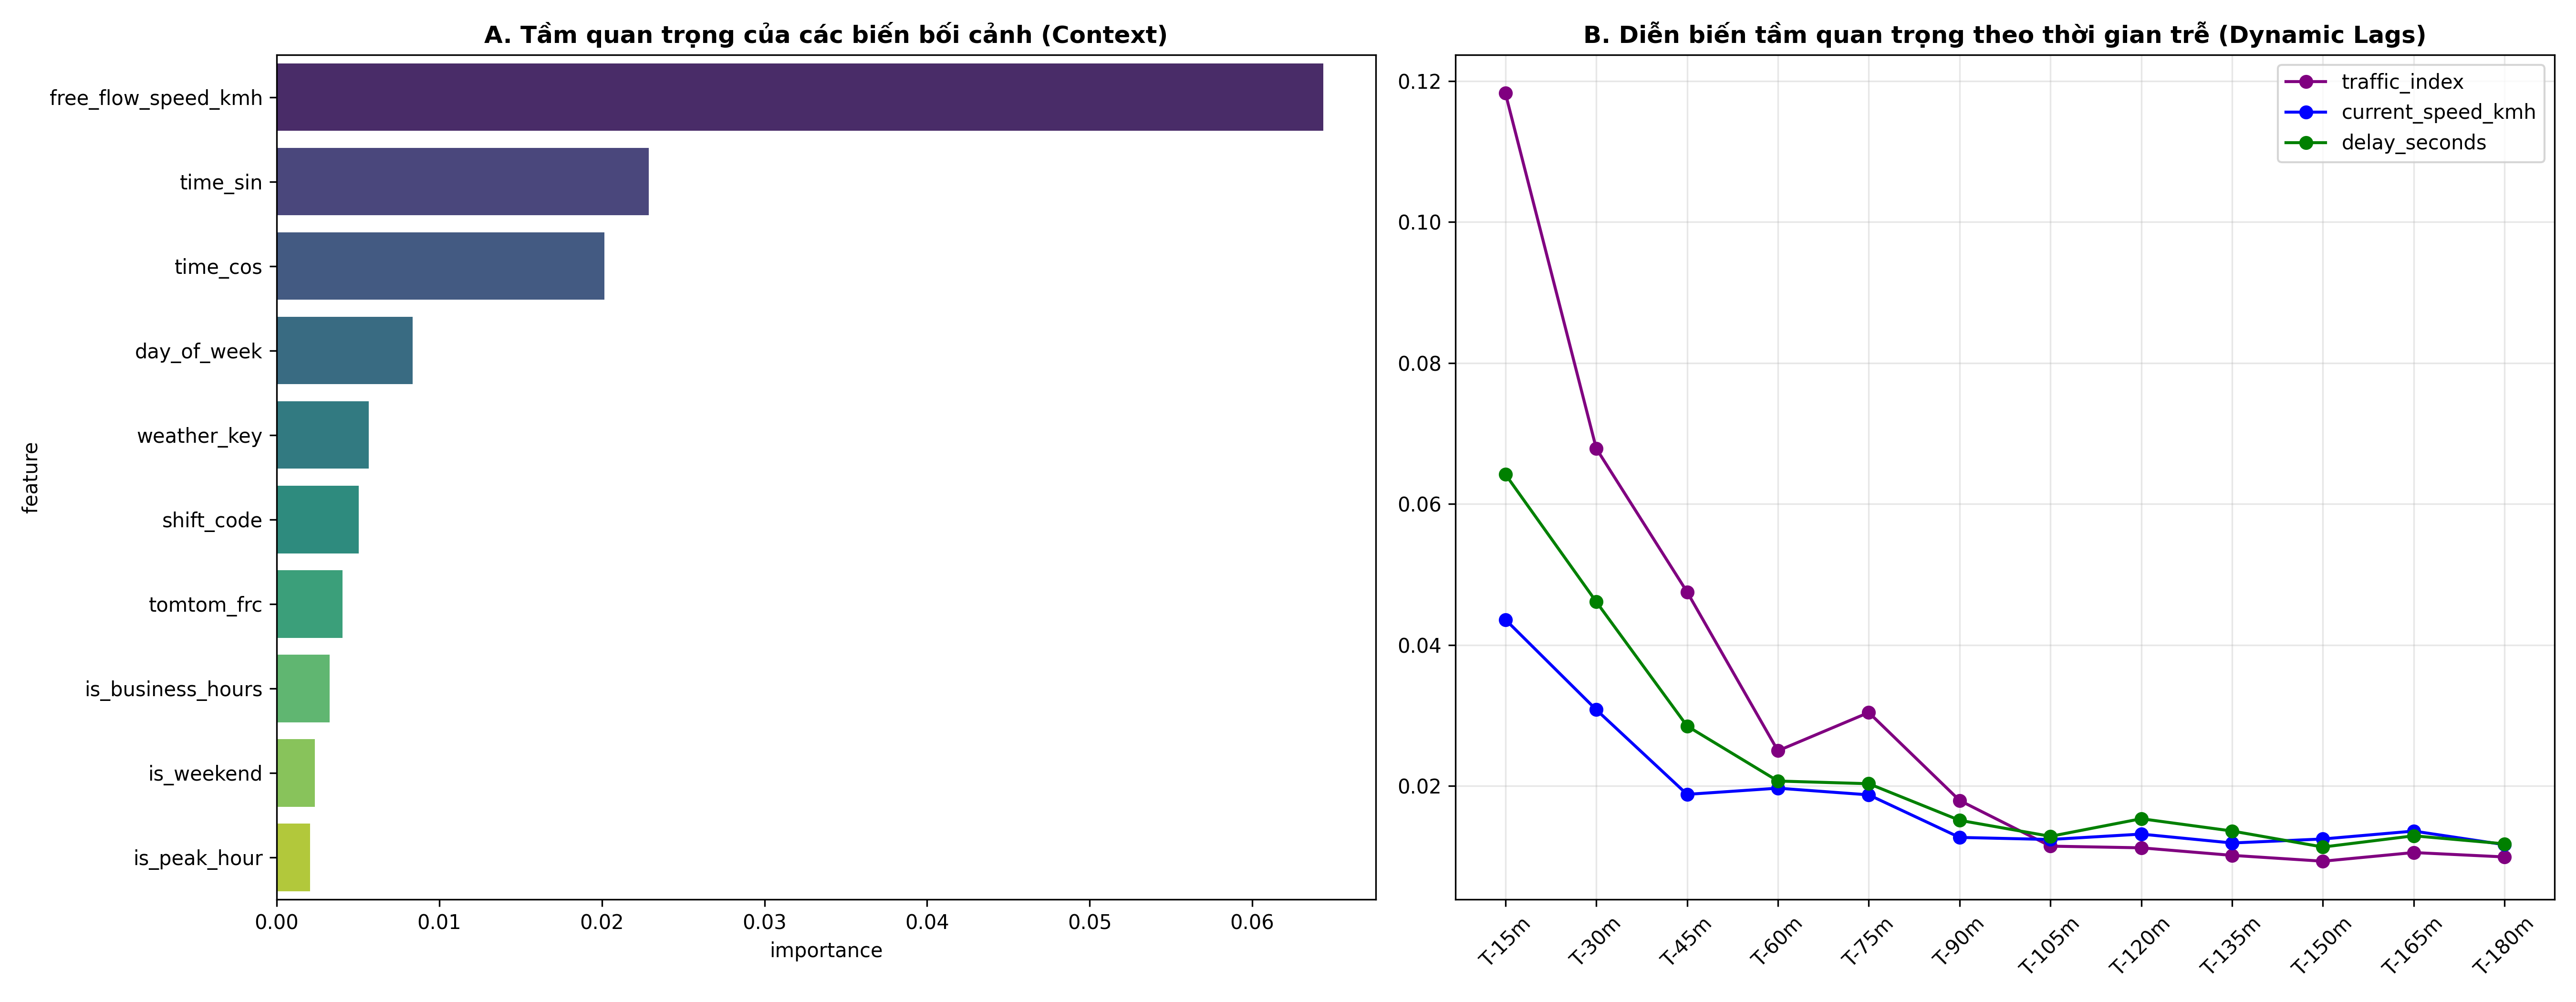
\includegraphics[width=0.8\textwidth]{Images/CH5/10.png}
    \caption{Xếp hạng mức độ đóng góp của các đặc trưng dựa trên Gini Importance (Random Forest)}
    \label{fig:5_10}
\end{figure}
